\documentclass[asp1.tex]{subfiles}
\begin{document}

%\begin{flushleft}

\section{Hardware}
\subsection{Hardware von Computern}

\subsubsection{Grundfunktionen und Entwicklung}

Computer arbeiten prinzipiell nach dem EVA-Prinzip (\textbf{E}ingabe, \textbf{V}erarbeitung, \textbf{A}usgabe)

\begin{figure}[H]
    \begin{center}
        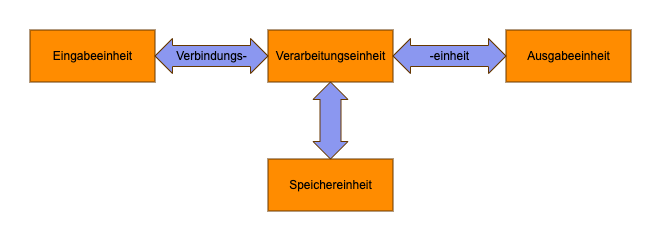
\includegraphics[width=1\textwidth]{EVA-Prinzip.png}
    \end{center}
    \caption{Grafische Darstellung EVA Prinzip}
\end{figure}

\textbf{Exemplarische Hardware:}

\begin{table}[H]
    \centering
    \begin{tabular}{l|l}
        Einheit              & Exemplarische Hardware             \\\hline
        Eingabeeinheit       & Tastatur, Maus, Mikrophon, Scanner \\
        Verarbeitungseinheit & CPU, GPU                           \\
        Ausgabeeinheit       & Monitor, Drucker, Lautsprecher     \\
        Speichereinheit      & HDD, SSD
    \end{tabular}
\end{table}

Computer werden heutzutage kaum noch als „Stand-alone-Geräte“/“Einzelplatzrechner“ benutzt, sondern sind firmenintern oder weltweit vernetzt. Trotzdem ist die Bezeichnung „PC – Personal Computer“ geblieben. Zusätzlich dazu gibt es noch weitere Bezeichnungen, die verschiedene Geräteklassen bilden:

\begin{longtable}{|p{0.15\textwidth}|p{0.4\textwidth}|p{0.323\textwidth}|}

    \hline
    \textbf{Bezeichnung}       & \textbf{Beschreibung}                                                                                                                                                                                                                                                                                                            & \textbf{Einsatzzweck}                                                                                                                                                                                                                                     \\\hline
    \textbf{Barebone}          & Meist würfelförmiges Gehäuse ca. 20x20x35 cm.
    Meist ist die Bestückung der Barebones nach Kundenwunsch
    möglich – von extrem sparsam bis zu durchschnittlichen
    Leistungen alles möglich.  & Einsatz als sparsamer Office-Rechner für die tägliche Arbeit bei geringem Platz und Stromverbrauch.                                                                                                                                                                                                                                                                                                                                                                                                                                                                                          \\\hline

    \textbf{Notebook}          & Mobiles Endgerät bei dem alle Komponenten inkl. Tastatur und Flachbildschirm untergebracht sind. Größe meist 35x28x3 cm. \newline Gutes Preis-Leistungsverhältnis. \newline Hardware sitzt meist „unter“ der Tastatur.                                                                                                           & Hoch mobiles arbeiten in verschiedenen Anwendungen – häufig in Verbindung mit Docking-Station um in Büros schnell konfigurierbare und flexible Arbeitsplätze zu schaffen.                                                                                 \\\hline

    \textbf{Netbook}           & Mobiles Endgerät bei dem alle Komponenten inkl. Tastatur und Flachbildschirm untergebracht sind. Größe meist 25x18x2 cm und damit kleiner als ein Notebook/Laptop. Dafür geringere Leistung als ein Notebook. \newline Hardware sitzt meist „unter“ der Tastatur.                                                                & Hoch mobiles Arbeiten, meist in Office-Anwendungen. Mobilität steht noch mehr im Fokus als beim Notebook. Dafür nimmt die Leistung und damit die Fähigkeit zum Einsatz als Büroarbeitsplatz ab.                                                           \\\hline

    \textbf{Tablet}            & Mobiler PC mit sehr flachem Gehäuse (<2 cm) und integriertem Display (Touch- und Stifteingabe). Meist keine Tastatur (außer bei hybriden Geräten). \newline Hardware sitzt „unter“ dem Display und es sind mobile Betriebssysteme im Einsatz.                                                                                    & Mobiles Arbeiten – selten die Eingabe von Daten, eher das Präsentieren von Informationen beim Kunden (z.B. im Außendienst – Marketing/Verkauf). \newline Sonderfälle wie z.B. Tablets zum Zeichnen und modellieren oder Branchenlösungen (Kassensysteme). \\\hline

    \textbf{Smartphone}        & Mobiler PC mit sehr flachem und kleinem Gehäuse und integriertem Display (Touch- und Stifteingabe). Leistungsschwächeres Tablet.                                                                                                                                                                                                 & Mobile Kommunikation (z.B. Mails oder Telefonate) bereitstellen. Daten einsehen, jedoch nur selten verarbeiten.                                                                                                                                           \\\hline

    \textbf{Wearable Computer} & tragbare Kleinstcomputer, die direkt am Körper getragen werden. Die meiste Zeit sind sie nur im Hintergrund tätig. Beispiele sind Smartwatches oder Datenbrillen.                                                                                                                                                                & Mobile Kommunikation, Überwachung von Körperfunktionen, bereitstellen von Informationen.                                                                                                                                                                  \\\hline

    \textbf{Desktop-PC}        & Flexible Konfiguration der Hardware in allen Facetten möglich. D.h. freie Wahl von Betriebssystem, Hardware und Größe des Gehäuses. \newline Leistungsfähigkeit schwankt stark aufgrund der flexiblen Hardware. \newline Eingabe – und Ausgabegeräte sind nicht fest verbaut, sondern werden über I/O-Schnittstellen angebunden. & Alles, außer mobiles Arbeiten. \newline Je nach Leistung von reiner Office-Tätigkeit bis hin zum rendern oder compilieren von Code ist alles möglich.                                                                                                     \\\hline

    \textbf{Industrie-PC}      & Speziell für Aufgaben im industriellen Bereich eingesetzt. Verarbeitung von Prozessdaten in Echtzeit steht im Vordergrund (z.B. Überwachung einer Produktionsmaschine). \newline Häufig so ausgelegt, dass sie Temperatur-, Schock- und Wasserresistent sind.                                                                    & Steuerung und Überwachung von Industrieanlagen.

    \\\hline
\end{longtable}

\break

\subsubsection{Hersteller und Leistungsmerkmale}

\textbf{Das Leistungsportfolio im IT-Bereich}

Die Datenverarbeitung in Unternehmen verfolgt unterschiedliche Ziele und wird unterschiedlich ausgelebt. In einigen Betrieben gilt die Datenverarbeitung als Mittel zum Zweck, in anderen ist sie eine Kernkompetenz und Verkaufsmerkmal.
Je nach Ziel der Datenverarbeitung gilt es, die passende Geräteklasse von einem entsprechenden Hersteller und zur Aufgabe passenden Leistungsmerkmalen anzuschaffen.

\textbf{Ziele der Datenverarbeitung}
\begin{itemize}
    \item   Schneller Verarbeitung großer Datenmengen
    \item   Beseitigung monotoner Routinetätigkeiten
    \item   Verbesserung und Automatisierung der Arbeitsabläufe
    \item   Bessere Individualisierung und Automatisierung durch Entscheidungssysteme, autonome und intelligente Unterstützungssysteme
    \item   Mehr und schnellere Informationen über Vorgänge (besseres Informationssystem)
    \item   Bessere Kommunikation durch die Integration und Vernetzung von Aufgaben und Funktionen
    \item Höhere Wirtschaftlichkeit durch geringere Personal- und Sachkosten

\end{itemize}

\begin{longtable}{|l|p{6cm}|p{6cm}|}
    \hline
    \textbf{Geräteklasse}    & \textbf{Bekannte Hersteller}                                     & \textbf{Leistungs-/Entscheidungsmerkmale}                                                                                                                                                                                                                                      \\\hline

    \textbf{Barebone}        & Intel, Gigabyte, Dell, Fujitsu, Hyundai, HP                      & Leise/Passive Kühlung (Sone), Preis, Stromverbrauch (Watt), Gehäusegröße, vorgefertigte Konfiguration (Massenbestellungen möglich?), Leistung (Anzahl Kerne; Taktfrequenz von CPU, RAM und ggf. GPU; Speicherplatzmenge RAM, Anzahl Anschlüsse)                                \\\hline

    \textbf{Desktop-PC}      & HP, Dell, Intel, Apple, Medion                                   & Preis, Grafikkartenleistung (VRAM, Taktung), CPU-Leistung (Taktung, Anzahl der Kerne, Overclocking möglich?), RAM, Konnektivität (HDMI/Display Port, USB, Ethernet), Kühlung(Lautstärke; Wasser oder Luft), Speicher (Kapazität, SSD/HDD), Stromverbrauch, Nachrüsten möglich? \\\hline

    \textbf{Notebook/Laptop} & Acer, HP, Dell, Lenovo, Asus, Apple, MSN                         & Preis, Mobilität/Akkulaufzeit, Konnektivität (Ethernet vorhanden?), Bildschirm (Auflösung, Bildwiederholrate), Grafikkartenleistung (VRAM, Taktung), CPU-Leistung (Taktung, Anzahl der Kerne), RAM, Konnektivität (HDMI/Display Port, USB, Ethernet)                           \\\hline

    \textbf{Netbook}         & Lenovo, Panasonic, Google, Microsoft                             & Preis, Mobilität/Akkulaufzeit, Konnektivität (Ethernet vorhanden?), Bildschirm (Auflösung, Bildwiederholrate), Grafikkartenleistung (VRAM, Taktung), CPU-Leistung (Taktung, Anzahl der Kerne), RAM, Konnektivität (HDMI/Display Port, USB, Ethernet)                           \\\hline

    \textbf{Tablet}          & Samsung, Apple, Microsoft, Lenovo                                & Preis, Mobilität/Akku, Bildschirmauflösung, Betriebssystem, Display, Kamera                                                                                                                                                                                                    \\\hline

    \textbf{Smartphone}      & Samsung, Apple, OnePlus, Google, Nokia, Huawei, Sony, Blackberry & Preis, Mobilität/Akku (Ladezeiten), Fingerabdrucks Sensor, Design, Konnektivität (AUX?), Betriebssystem, Display, Kamera                                                                                                                                                       \\\hline

    \textbf{Industrie-PC}    & OnLogic, Siemens, Histton                                        & Preis, Staubschutz, Temperaturbeständigkeit                                                                                                                                                                                                                                    \\\hline

    \textbf{Wearables}       & Apple, Samsung, Huawei, Epson, Microsoft, Fossil                 & Preis, Akkuleistung, Funktionen(Körperfunktionen tracken, Sensoren), Design

    \\\hline
\end{longtable}

\break

\subsubsection{Ergonomie am Arbeitsplatz}

\textbf{Ergonomie} ist eine wissenschaftliche Disziplin, die sich mit der menschlichen Arbeit befasst. Konkret stellt sie sich die Frage, wie ein Arbeitsplatz gestaltet sein muss, um eine perfekte Symbiose aus Menschen und Arbeitsmitteln (hierzu gehören im Übrigen auch Maschinen und Werkzeuge) herzustellen. Auch die Inhalte der Arbeit, das allgemeine Umfeld am Arbeitsplatz und die Organisation sind wichtige Aspekte, die alle ihren Anklang in der Ergonomie finden und berücksichtigt werden müssen. Die Gesundheit – sowohl körperliche als auch geistige – steht in jedem Fall klar im Vordergrund.

Faktoren, die bei der täglichen Arbeit auf eine Person einwirken:
\begin{itemize}
    \item Langes Sitzen und schlechte Körperhaltung
    \item Blaulicht intensive Arbeit am Bildschirm
    \item Ermüdung der Augen durch langes betrachten des Bildschirms
    \item Schlechte oder zu „gute“ Belüftung des Arbeitsplatzes
    \item Lärm am Arbeitsplatz (Nebengeräusche)
    \item Wenig natürliches Licht
    \item Schlechte IT-Ausstattung
    \item Schlechte Ergonomie der Tastatur/Maus
    \item Generell zu lange Verwendung - egal von was
    \item Geräte mit großer Strahlung
    \item Überarbeitung und dadurch Folgeeffekte wie Schlafmangel und schlechte Ernährung
    \item Staub und Feinstaub
\end{itemize}


Möglichkeiten, die Belastung bei der Arbeit am Computer möglichst gering zu halten:

\begin{itemize}
    \item Häufiges Wechseln der Sitzposition
    \item Anlehnen mit dem gesamten Rücken vermeiden – trotzdem aufrecht sitzen
    \item Sitzhöhe so, dass die Füße auf dem Boden stehen, Arme und Beine möglichst im rechten Winkel
    \item Höhenverstellbare Schreibtische (der das Arbeiten im Stehen ermöglicht)
    \item Höhe des Monitors, der obere Rand sollte auf Höhe der Augen sein
    \item Abstand Monitor zum Benutzer (das 1,2-Fache der Diagonale in cm)
    \item Verwendung von Blaulichtfiltern beim Monitor (ggf. auch über das Betriebssystem)
    \item Ggf. Brillen mit Blaulichtfiltern
    \item Soweit wie möglich auf Kontrast achten (wenn möglich: Dark Mode)
    \item Regelmäßige Bildschirmpausen (Aufstehen, Bewegen)
    \item Sport treiben, um die Muskulatur zu stärken
    \item Regelmäßiges lüften oder wenn nichts Anderes möglich ist, Luftfilter verwenden
    \item Gesundes Essen und Trinken
    \item Wenn möglich „Schallarme“ Räume
    \item Grüne Büros (Pflanzen)
    \item Gute Beleuchtung (ggf. mit Lampen, die Sonnenlicht nachbilden – Stichwort Vitamin D)
    \item Gutes Zeitmanagement
    \item Tastatur möglichst ebenerdig und ggf. mit Handballenauflagen
    \item Verwendung von ergonomischen Mäusen und Tastaturen
\end{itemize}

\subsubsection{Green IT und Wirtschaftlichkeit}

\textbf{Green-IT} ist ein Leitbegriff zur Schaffung einer Unternehmenskultur, die IT möglichst umweltschonend beschafft und einsetzt. Entscheidender Grundgedanke der Green-IT ist eine ganzheitliche Betrachtungsweise. Beschaffung, Nutzung, Verwertung und Entsorgung von IT werden als Teil eines zusammenhängenden Kreislaufes verstanden.
Dafür gibt es verschiedene Richtlinien, Nachhaltigkeitskonzepte und jährliche Nachhaltigkeitsberichte.

\textbf{Beispiele für Umwelt- und Prüfzeichen:}

\begin{table}[H]
    \centering
    \begin{tabular}{|p{0.5\textwidth}|p{0.5\textwidth}|}
        \hline

        \begin{wrapfigure}{l}{0.25\textwidth}
            
\includegraphics{energystar.png}
        \end{wrapfigure}

        Weltweit verbreitet
        Zertifiziert die Energieeffizienz von Hardware
        Stammt aus den USA
        Hersteller können das Siegel nach Anfrage anbringen. Die Einhaltung wird aber zunächst nicht kontrolliert.
        Es erfolgen stichprobenartige Kontrollen.

         &

        \begin{wrapfigure}{l}{0.25\textwidth}
            
\includegraphics{tuvrheinland.png}
        \end{wrapfigure}

        TÜV Rheinland ist als unabhängiges Prüfunternehmen von der Zentralstelle der Länder für Sicherheitstechnik für die Zertifizierung von vielen Produktgruppen zugelassen.
        Ein zertifiziertes Produkt hat bestimmte Prüfungen des TÜV Rheinland – beispielsweise auf Sicherheit und Qualität – erfolgreich bestanden.

        \\\hline

        \begin{wrapfigure}{l}{0.25\textwidth}
            
\includegraphics{ecolabel.png}
        \end{wrapfigure}

        Europaweit anerkanntes Umweltzeichen für Waren und Dienstleistungen.
        Heute vergeben Prüfinstitute das EU-Ecolabel im Auftrag der Umweltministerien der teilnehmenden europäischen Länder.

         &

        \begin{wrapfigure}{l}{0.25\textwidth}
            
\includegraphics[width=\linewidth]{tco.jpg}
        \end{wrapfigure}

        Zertifikat, dass die Ergonomie und die Produktlebensdauer eines Produktes bewertet.
        Vergeben wird es durch den schwedischen Dachverband der Angestellten- und Beamtengewerkschaft.
        Kontrolle erfolgt Stichprobenartig.

        \\\hline
    \end{tabular}
\end{table}

\break

\textbf{Maßnahmen für verschiedene Aspekte von Green-IT:}
\begin{table}[H]
    \centering
    \begin{tabular}{|p{0.3\textwidth}|p{0.7\textwidth}|}

        \hline

        Bedarfsgerechter Einsatz von Hardware und Software prüfen                                         & Einsatz von IT-Hardware (z.B. Rechner und Peripheriegeräten) auf korrekte Dimensionierung prüfen

        \\\hline

        Einsparung Energie und Energiekosten durch effiziente IT-Lösungen                                 & Anschaffung von Energieeffizienten Produkten (Energieeffizienzklasse A)
        \newline Abwärme nutzen?! Z.B. Abwärme von Servern in den „Heizkreislauf“ einspeisen.
        \newline Virtualisierung

        \\\hline

        Beratung, den Lebenszyklus der Geräte zu verlängern, Kosten zu senken, Refurbished IT einzusetzen & Extreme Temperaturen und Umgebungseinflüsse und Leistungsszenarien vermeiden
        \newline Bei der Anschaffung auf zukünftige Performance achten
        \newline Auf Möglichkeiten zum Um-, Nach und Aufrüsten achten
        \newline Hardware im Unternehmen weitergeben (z.B. bei Neuanschaffung alte Geräte an Mitarbeiter geben, die weniger Leistung benötigen)
        \newline Bring Your Own Device (BYOD) prüfen

        \\\hline

        Bedarfsgerechter Betrieb der IT anstelle eines durchlaufenden Betriebs                            & Auf Standby verzichten, wenn möglich
        \newline PC, Monitor und co in Energiesparmodus und wenn möglich ganz ausschalten
        \newline WLAN über Nacht deaktivieren
        \newline Licht o.ä. an Zeit oder Sonnenstand knüpfen

        \\\hline

        Energie und Kosten durch Virtualisierung sparen                                                   & Betriebssysteme, Server und Entwicklungsumgebungen virtualisieren, um Kosten für redundante Systeme zu sparen.

        \\\hline

        Einsatz umweltschonender Verbrauchsmaterialien                                                    & Einsatz gebrauchten Geräten
        \newline Auf korrekte Mülltrennung bei der Entsorgung von Elektroschrott achten
        \newline Generell recycelte Produkte kaufen
        \newline So weit wie möglich papierlos arbeiten
        \newline Einsatz von grünem Strom

        \\\hline

        Software auf Nachhaltigkeit prüfen, eventuell Open-Source-Software vorziehen                      & Open-Source-Software ist häufig anpassbar und kann somit an die eigenen Anforderungen angepasst werden.
        \newline Der Funktionsumfang ist zwar häufig geringer aber kann ausreichend sein und ist meistens mit geringeren Hardwareanforderungen verbunden.
        \newline Die Software wird häufig durch eine große Community unterstützt und kann so auf alten System lauffähig und sicher gehalten
        \newline Bei der Anschaffung von neuer Software (egal ob Open-Source oder gekauft) sollten die Hardwareanforderungen und die Passung mit dem restlichen System beachten werden.

        \\\hline

        Mitarbeiter auffordern, umweltfreundlicher zu kommunizieren                                       & Möglichst auf Papier etc. verzichten.
        \newline Lokale Kommunikationssysteme sollten bevorzugt werden.
        \newline Wenn möglich Dienstreisen durch virtuelle Konferenzen ersetzen.



        \\\hline
    \end{tabular}
\end{table}

\subsubsection{Zentraleinheit, Mainboard, Betriebssystem unterscheiden}

Grundlage eines jeden Computers ist die Zentraleinheit. Sie besteht im engeren Sinne aus dem Mainboard und den direkt darauf bestückten Komponenten. Dazu zählen CPU und RAM.
Da RAM-Speicher flüchtig ist und beim Abschalten des Computers gelöscht wird, wird im ROM (Read-Only-Memory) auf dem Mainboard ein Grundprogramm als Grundbetriebssystem oder BIOS (Basic-Input-Output-System, auch UEFI) gespeichert.

Damit alle Operationen konfliktfrei ablaufen können, wird ein Takt vom auf dem Mainboard liegenden Taktgeber (Clock, CLK) vorgegeben.

Das BIOS führt den Startvorgang aus und ruft das Betriebssystem auf, welches auf einem externen Speicher liegt.
BIOS wird durch das schnellere, leistungsfähigere und mit besserem GUI ausgestattete UEFI (Unified Extensible Firmware Interface) abgelöst. EUFI ist im Gegensatz zum BIOS ein eigenes 64-Bit Betriebssystem, es können also Updates geladen werden.

Je nach Hersteller kann das BIOS/UEFI durch das Drücken der Tasten Entf, F1, F2, F8, F10, ESC, … während des Startvorgangs aufgerufen werden.


\subsubsection{Mainboard}

Das Mainboard ist die Hauptplatine des Computers. Alle Hardwarekomponenten sind auf ihm angebracht oder verbaut.

Abmessungen des Mainboards sind im mobilen Bereich sehr individuell auf das Gerät angepasst, aber folgen für Desktop-PCs im Normalfall dem ATX-Formfaktor (Advanced Technology Extended). Merkmale des \textbf{ATX-Formfaktors}:

\begin{itemize}
    \item Festgelegte Größe
    \item Vorgeschriebene Anordnung von Befestigungslöchern
    \item Board ist in verschiedene Bereiche aufgeteilt, welche eine maximale Höhe vorgegeben haben
    \item Anordnung und Art der Anschlüsse sind genormt
\end{itemize}

\textbf{Komponenten auf dem Mainboard:}
\begin{itemize}
    \item Sockel (physikalische Verbindung zwischen Mainboard und CPU)
    \item Chipsatz (Vermittlung der Daten zwischen Input- und Output-Controller)
    \item IC für das UEFI
    \item Batterie für die Systemuhr (wenn Mainboard vom Strom getrennt)
    \item Steckplätze für RAM
    \item Steckplätze für Erweiterungskarten
    \item Schnittstellenanschlüsse
    \item Anschluss für die Spannungsversorgung
\end{itemize}

\break
\textbf{Begriffserklärungen:}
\begin{table}[H]
    \centering
    \begin{tabular}{|p{0.3\textwidth}|p{0.7\textwidth}|}
        \hline

        \textbf{Begriff} & \textbf{Beschreibung} \\\hline

        \textbf{Schnittstellen}
        \newline (Welche finden sich an einem Mainboard)
                         &
        PCI-E, (Reset-, HDD, Power), Audio-Anschlüsse, Display-Port, USB-Ports, E-Sata-Ports, PS2-Ports, VGA, DVI, HDMI, Netzwerkanschlüsse, Firewire

        \\\hline

        \textbf{Chipsatz}
        \newline (Welche Chipsätze sind derzeit für AMD und Intel relevant)
                         &
        Das zentrale Element auf einem Motherboard ist der Chipsatz (engl. Chipset). Zwar ist der Hauptprozessor das schlagende Element in einem Computer, aber der Chipsatz sorgt erst dafür, dass die verschiedenen Komponenten miteinander kommunizieren und arbeiten können. Der Chipsatz ist das Bindeglied zwischen den einzelnen Komponenten eines Computers. Egal was in einem Computer passiert, der Chipsatz ist immer daran beteiligt.
        \newline AMD – x570, B550, B550a
        \newline Intel – B460, H470, Z490

        \\\hline

        \textbf{Steckplätze für Erweiterungskarten}
        \newline (Welche Anschlüsse/Standards gibt es derzeit auf Mainboards)
                         &
        PCI, PCI-E (x4 bis x16), M.2 (z.B. für SSD), SATA, USB, ggf. RAM-Steckplätze, ggf. PWM-Steckplätze

        \\\hline

        \textbf{SATA-Anschlüsse }
        \newline (was versteht man darunter)
                         &
        Serial Advanced Technology Attachment \textrightarrow \space Für Massenspeicher wie Festplatten, SSDs, DVD-Laufwerke, … (600 Mbyte/s)

        \\\hline

        \textbf{Sockel}
        \newline (welche Sockel sind derzeit in Verwendung)
                         &
        AMD: AM4, AM3+, STR4(für Threadripper)
        \newline Intel: LGA1151, LGA1200, LGA1155, LGA1151v2

        \\\hline
    \end{tabular}
\end{table}

\subsubsection{Anschlüsse und deren Verwendung}

\begin{outline}
    \1 PCIe-Steckplatz (PCI-Express)
    \2 Schnelle, Interne Schnittstelle für Erweiterungskarten
    \2 Eignet sich grundsätzlich für die Verbindung mehrerer Server und Baugruppen zu einem Computersystem
    \2 Geeignet für zeitkritische Anwendungen wie Bild- oder Tonwiedergabe
    \2 Sowohl für Kupferleitungen als auch für optische Verbindungen vorgesehen
    \2 PCIe Halbleiterschaltungen werden abgewandelt auch für DisplayPort, SATA und SAS verwendet
    \2 Verfügt über verschiedene Slots (x1, x4, x8 und x16). Dabei stehen die Zahlen für die Anzahl der in dem Slot kaskadierten Lanes
    \2 Grundsätzlich funktionieren kurze Karten auch in langen Slots
    \2 WICHTIG: mechanische Länge sagt nichts über die Anzahl der Lanes eines Slots aus
    \1 SATA (Serial-ATA)
    \2 Schnittstelle zum Anschluss von Massenspeichern
    \2 Blaue SATA-Buchsen sind mit 6 Gbit/s zurzeit die schnellsten
    \2 Ist wie USB abwärtskompatibel
    \2 Rote und Schwarze SATA-Buchsen setzen je nach Hersteller unterschiedliche Spezifikationen um (z.B. RAID-Unterstützung)
    \1 USB (Universal Serial Bus)
    \2 Universelle Schnittstelle für Peripheriegeräte
    \2 Lässt sich durch Steckkarten oder USB-Hubs fast beliebig erweitern
    \2 Identifikation der Geräte wird vom USB-Hostadapter im Computer durchgeführt
    \2 Hot-Plugging und Plug-and-Play möglich
    \2 Abwärtskompatibel
    \2 Zu USB zählt auch Firewire (mittlerweile eher selten verwendet) und Thunderbolt
    \2 Thunderbolt fasst in einer Steckverbindung USB, DisplayPort und PCIe zusammen und erreicht eine Geschwindigkeit von 10, 20 oder 40 Gbits/s
    \1 M.2-Port
    \2 Slot-artige Steckverbindung die für streifenförmige SSDs gedacht ist
    \2 Löst den mSATA-Anschluss ab
    \1 Lüfteranschlüsse
    \2 Entweder 3-Pin Anschlüsse (DC-Control: Kontrolle der Geschwindigkeit über die Spannung) oder 4-Pin Anschlüsse (Kontrolle der Geschwindigkeit mit PWM-Signal auf 4tem Pin)

\end{outline}

\subsubsection{CPU Grundlagen}

Der \textbf{Prozessor} bzw. Hauptprozessor (\textbf{CPU} – \textbf{C}entral \textbf{P}rocessing \textbf{U}nit) ist das Kernstück und die zentrale Verbindungseinheit eines Rechners.
Besteht aus mehreren Milliarden Transistoren, die auf einem Mikrochip angebracht sind – wird daher auch \textbf{Mikroprozessor} genannt.
Der eigentliche Mikrochip wird als \textbf{Prozessor-Die} bezeichnet und ist wesentlich kleiner als die Prozessorplatine. Die Größe des Prozessors wird maßgeblich durch die Anzahl der Kontakte bestimmt.

Die CPU holt nacheinander Befehle aus dem Speicher und veranlasst Informationsverarbeitung, Steuerung und Kontrolle der Systeme.

\textbf{Grundlegende Funktionsblöcke einer CPU:}

\begin{table}[H]
    \centering
    \begin{tabular}{|p{0.3\textwidth}|p{0.7\textwidth}|}
        \hline

        \textbf{Instruction Decode Unit (IDU)} & Befehlsdecoder; übersetzt die Befehle, die dem Prozessor als Programm übergeben werden, anhand eines prozessorientierten ROMs in Microcode und übergibt sie der Ausführungseinheit.

        \\\hline

        \textbf{Execution Unit (EXU)}          & Ausführungseinheit; führt die im Mikrocode vorliegenden Befehle aus.

        \\\hline

        \textbf{Control Logic (COL)}           & Kontrolleinheit; steuert den Ablauf der Mikroprogramme.

        \\\hline

        \textbf{Internal ROM}                  & Interner ROM-Speicher; beinhaltet die Mikroprogramme des Prozessors

        \\\hline

        \textbf{Bus Interface Logic (BIL)}     & Bussteuereinheit; Schnittstelle zwischen den internen Verbindungen und der Verbindung zum Chipsatz.

        \\\hline

        \textbf{Arithmetic Logic Unit (ALU)}   & Arithmetisch logische Einheit; führt arithmetische und logische Rechenoperationen aus.

        \\\hline

        \textbf{Floating Point Unit (FPU)}     & Fließkomma-Rechner/Co-Prozessor; führt Berechnungen mit Gleitkommazahlen aus.

        \\\hline

        \textbf{Data Cache (DC)}               & Cache-Speicher für Daten

        \\\hline

        \textbf{Code Cache (CC)}               & Cache-Speicher für Befehle; schneller Zwischenspeicher für Befehle.

        \\\hline
    \end{tabular}
\end{table}

\break

\textbf{Wichtige Begriffe:}
\begin{longtable}{|p{0.3\textwidth}|p{0.7\textwidth}|}
    \hline

    \textbf{AMD}                           & AMD entwickelt und vertreibt Computerchips, Mikroprozessoren, Chipsätze, Grafikprozessoren (GPUs) und System-on-a-Chip-Lösungen (SoC).
    \newline AMD hat keine eigene Herstellung, sondern vergibt die Produktion an Auftragshersteller.

    \\\hline

    \textbf{Intel}                         & Entwickler und Hersteller von Prozessoren für Desktop, Laptop und Servern. Außerdem Grafikchips und z.B. Desktop-PCs.

    \\\hline

    \textbf{TSMC}                          & Die Taiwan Semiconductor Manufacturing Company, Limited ist nach Intel und Samsung der weltweit drittgrößte Halbleiterhersteller und der weltweit größte unabhängige Auftragsfertiger für Halbleiterprodukte.

    \\\hline

    \textbf{Prozessorarchitektur}          & Unter Architektur versteht man bei Mikroprozessoren das technische Prinzip bzw. das Verfahren, nachdem Daten und Programme verarbeitet werden. Man unterscheidet CISC- und RISC-Prozessoren.CISC – Complex Instruction Set Computing (meist x86-Architekturen) RISC – Reduced Instruction Set Computing (meist ARM-Architekturen)Die Generationen einer CPU wie z.B. Tiger Lake oder Zen 3 können auch als Mikroarchitektur bezeichnet werden. Dabei dreht es sich um den genauen Aufbau einer CPU auf Ebene des Schaltblockplans.

    \\\hline

    \textbf{Strukturgröße}                 & Bezeichnet die Flächennutzung in Nanometern bei Chips. Derzeit sind 7nm bei AMD und 10-14nm bei Intel in Verwendung. Je kleiner die nm-Angabe ist, desto leistungsstärker und energieeffizienter ist der Chip.

    \\\hline

    \textbf{Cache}                         & Besonders schneller Zwischenspeicher, der direkt mit der CPU verbunden ist und die CPU durch Speicherung der wartenden Prozesse und Daten entlastet. Es gibt normalerweise 3 Größen L1, L2 und L3-Cache, wobei L1 der kleinste und L3 der größte Speicher ist. L1 befindet sich direkt am Kern (jeder Kern 1 Cache) L3-Cache wird meist zwischen allen Kernen geteilt.

    \\\hline

    \textbf{Taktfrequenz}                  & Die Taktfrequenz misst die Anzahl der Takte oder Zyklen, die von der CPU pro Sekunde durchgeführt werden in GHz (Gigahertz). Eine CPU mit einer Taktfrequenz von 3,2 GHz führt pro Sekunde 3,2 Milliarden Takte aus. Ganz allgemein lässt sich sagen, dass ein höherer Takt besser ist.

    \\\hline

    \textbf{Parallelisierung}              & Parallele Abarbeitung von verschiedenen Befehlen durch z.B. Mehrkernprozessoren (mehrere Rechenkerne auf einer CPU – z.B. Ryzen 5800 hat 8 baugleiche Rechenkerne). Häufig findet man Mehrkernprozessoren in Verbindung mit Multi-Threading (SMT bei AMD und Hyper-Threading bei Intel). Das bedeutet, es werden in einem Kern parallel mehrere Befehle/Programmabläufe (Threads) bearbeitet.

    \\\hline

    \textbf{Turbo Boost / Precision Boost} & Automatische Übertaktung der CPU bzw. einzelner Kerne bei Intel (Turbo) und AMD (Precision). Je nach thermischer und spannungsbedingter Reserve und nach Arbeitslast der restlichen Kerne wird der Takt eines Kerns bis zur maximalen Grenze erhöht, um kurzzeitig die Verarbeitung der Daten zu beschleunigen.

    \\\hline

    \textbf{TDP}                           & Thermal Design Power – gibt die maximale abgegebene Wärmeleistung eines Prozessors in Watt an. Liegt unter der tatsächlichen Spannung, gibt aber einen Hinweis auf den Verbrauch des Systems. TDP verschiedener Hersteller lassen sich aufgrund unterschiedlicher Messparameter nicht miteinander vergleichen. Neben dem Verbrauch gibt die TDP auch einen Hinweis auf die Dimensionierung des Kühlers. Je größer desto besser sollte das Kühlsystem sein (Passiv, Luft, Wasserkühlung).

    \\\hline

    \textbf{GPGPU}                         & General Purpose Computation on Graphics Processing Unit – Schnittstelle mit der Möglichkeit, allgemeine Berechnungen auf die GPU auszulagern. Notwendig, bei Systemen, bei der ein Grafikchip in die CPU integriert ist.

    \\\hline
\end{longtable}

\subsubsection{CPU Leistungsmerkmale}

\begin{outline}
    \1 CPU-Takt
    \2 Geschwindigkeit, mit der der Prozessor arbeitet
    \2 In Megahertz (MHz) oder Gigahertz (GHz) angegeben
    \2 Frequenz mit der der Prozessor laut Hersteller getaktet ist
    \1 Anzahl der Prozessorkerne
    \2 Durch Mehrkernprozessoren wird die Leistungsfähigkeit gesteigert
    \2 Mehrkernprozessoren bestehen aus zwei oder mehr gleichen Prozessorkernen auf einem einzigen Mikrochip
    \2 Kerne können gleichzeitig unterschiedliche Prozesse abarbeiten oder parallel einen einzigen Prozess ausführen
    \2 Kerne haben ihren eigenen Takt
    \2 \textrightarrow Weitere Merkmale: Takt des einzelnen Kerns und maximale Taktrate aller Kerne zusammen („All-Core-Boost“)
    \1 Geschwindigkeit, mit der Daten zum Prozessor übertragen werden
    \2 Abhängig von Taktung und Verbindungsart der Datenleitung
    \2 Es existieren verschiedene Varianten (Front Side Bus, QuickPathInterconnect, HyperTransport, Direct Media Interface, Unified Media Interface)
    \1 MIPS
    \2 \textbf{M}illions of \textbf{I}nstructions \textbf{p}er \textbf{S}econds
    \1 FLOPS
    \2 \textbf{F}loating \textbf{P}oint \textbf{O}perations \textbf{P}er \textbf{S}econd
    \2 Misst Leistungsfähigkeit anhand der Gleitkommazahlen-Operationen, die in einer Sekunde ausgeführt werden können
    \1 CISC
    \2 \textbf{C}omplex \textbf{I}nstruction \textbf{S}et \textbf{C}omputing
    \2 Häufig Bezeichnung für allround-Prozessoren, die einen komplexen Befehlssatz verarbeiten können
    \2 Bearbeitung eines Befehls kann mehrere Takte dauern, da ein komplexer Befehl aus mehreren kleinen Befehlen bestehen kann

    \break
    \break

    \1 RISC
    \2 \textbf{R}educed \textbf{I}nstruction \textbf{S}et \textbf{C}omputer
    \2 Kleinerer und effizienterer Befehlssatz
    \2 Meistens ein Befehl pro Takt
    \2 Aufgaben können effizienter und kleinschrittiger abgearbeitet werden
    \1 SIMD
    \2 \textbf{S}ingle \textbf{I}nstruction, \textbf{m}ultiple \textbf{d}ata; Rechnerarchitektur mit Vektorprozessoren, bei der viele Prozessoren ihre Befehle von einem Befehlsprozessor erhalten und gleichzeitig unterschiedliche Daten verarbeiten
    \1 Simultaneous Multithreading (SMT) / Hyper-Threading (HT)
    \2 SMT: Prozessor kann mehrere Threads gleichzeitig ausführen
    \2 HT: Intel SMT
    \1 Cachegröße
    \2 Für Effizienz des Cache ist Größe (je größer, desto besser) und Taktfrequenz entscheidend
    \1 Speicherbusse
    \2 Anzahl und Datenrate der unterstützten Speicherbusse – umso höher, desto besser
    \1 Befehlssatzerweiterung
    \2 Erweiterung des klassischen Befehlssatzes, der zusätzliche Befehle hinzufügt
    \2 Kann Leistungsfähigkeit erhöhen
\end{outline}

\textbf{CPU-Taktsteigerung:}
\begin{outline}
    \1 Eine CPU-Taktsteigerung (z.B. durch Boost-Funktionen oder Übertaktung) führt in der Regel zwar zu einer höheren Verarbeitungsgeschwindigkeit, allerdings steigt auch die Verlustleistung in Form von Wärme, die abgeführt werden muss. Dies liegt daran, dass für die Erhöhung der Taktrate meist auch die am CPU anliegende Spannung (Corespannung) erhöht werden muss. Das UEFI stellt die Corespannung in der Regel automatisch ein und überwacht diese im laufenden Betrieb. Je nach Energiespartechnik oder gewünschter Leistung wird die Spannung lastabhängig gesteuert oder einzelne Kerne komplett abgeschaltet.

    \1 Eine niedrigere Corespannung verringert die Leistungsaufnahme und die Abwärme einer CPU und ermöglicht dadurch höhere CPU-Taktraten.

    \1 Die Corespannung ist ab Werk auf eine „sichere“ Einstellung festgelegt, die für jeden Nutzer ausreichend ist. Sie kann manuell erhöht oder gesenkt werden, um z.B. den CPU zu übertakten oder die Leistungsaufnahme zu optimieren (undervolting).
\end{outline}

\textbf{Weitere wichtige Begriffe}
\begin{outline}
    \1 x64 und ARM sind die häufigsten Arten von Prozessoren
    \2 x64 \textrightarrow\space CISC \textrightarrow\space zielt auf höhere Leistung
    \2 ARM \textrightarrow\space RISC \textrightarrow\space zielt auf höhere Energieeffizienz
    \1 EIST-Verfahren
    \2 Enhanced Intel SpeedStep Technology
    \2 Energiesparfunktion von Intel, bei der Takt und Kernspannung dynamisch angepasst werden
    \2 Besonders relevant auch für Notebooks, da erkannt wird ob Betrieb per Akku oder Netzteil stattfindet
    \2 AMD Gegenstück heißt CoolnQuiet
\end{outline}

\subsubsection{RAM}

\begin{outline}
    \1 Random Access Memory
    \1 Wird auch als \textbf{Lese-Schreibspeicher oder Arbeitsspeicher} bezeichnet
    \1 Wird beim Herunterfahren des Endgerätes gelöscht \textrightarrow\space flüchtiger Speicher
    \1 Es wird zwischen \textbf{SRAM} und \textbf{DRAM} unterschieden
    \1 SRAM (Static Random Access Memory):
    \2 Speicherzellen aus Flipflops aufgebaut
    \2 Jedes Flipflop besteht aus sechs Transistoren und kann entweder 0 oder 1 als Zustand einnehmen
    \2 Durch einen kurzen Spannungsimpuls wird er Zustand eingenommen und unverändert gehalten, solange die Betriebsspannung anliegt
    \2 Sehr performant, kürzere Zugriffszeiten als bei DRAM
    \2 Höherer Platzverbrauch durch Flipflops \textrightarrow\space geringe Integrationsdichte (Speichereinheiten pro Flächeneinheit)
    \2 Teurer als DRAM
    \2 Wird für Cache-Speicher verwendet
    \1 DRAM (Dynamic Random Access Memory)
    \2 Überbegriff für alle dynamisch arbeitenden RAM-Bausteine
    \2 DRAM-Speicherzelle besteht typischerweise aus einem Transistor und einem Kondensator
    \2 Informationsspeicherung erfolgt durch Speichern einer Ladung im Kondensator
    \2 Da Ladung im Kondensator flüchtig ist, muss der Speicher regelmäßig aktualisiert werden (\textbf{refresh}), z.B. alle 32ms
    \2 DRAM ist günstiger und hat höhere Integrationsdichte
    \2 Wird als primärer Arbeitsspeicher eines PCs verwendet
    \1 DDR-SDRAM
    \2 Synchronous Dynamic Random Access Memory
    \2 Heutzutage in PCs verbaut
    \2 Daten werden synchron zum Speicher-Bus übertragen
    \2 Takt wird durch System-Bus vorgegeben
    \2 DDR: Double Data Rate \textrightarrow\space Daten werden im Vergleich zu SD-RAM doppelt so schnell übertragen, da sowohl bei ansteigender als auch bei abfallender Taktflanke übertragen wird (SD-RAM nur bei abfallender)
    \1 Verschiedene RAM-Typen je nach Anwendungsgebiet
    \2 Z.B.: DDR-3, DDR-4, DDR-5, GDDR
    \2 Unterscheiden sich durch maximale Taktraten, Aufbau und Datenübertragungsraten
    \2 DDR4: verbreitetste Variante
    \2 DDR5: Wird immer populärer, noch eher neue Technologie
    \2 GDDR: Ausschließlich verwendet im Grafikbereich (z.B. bei Grafikkarten)
    \2 \textbf{Verschiedene RAM-Typen sind untereinander nicht kompatibel!}
    \1 Formfaktoren
    \2 Man unterscheidet zwischen \textbf{Single-Sided-} und \textbf{Double-Sided-Modulen} (einseitig oder zweiseitig bestückt)
    \2 Größe und Anzahl der Kontakte sind je nach Aufbau und verwendeter Technologie unterschiedlich, aber sind durch \textbf{JEDEC} (Joint Electronic Device Engineering Council) festgelegt und für Hersteller einheitlich
    \2 Im Normalfall werden in Desktop-PCs \textbf{DIMM}-RAM (Dual Inline Memory Modul) Module verbaut. Anschlusskontakte beidseitig am Rand der Leiterplatte angebracht
    \2 Für Laptops oder kleine Computer gibt es SO-DIMM-RAM-Riegel. Das sind kleinere DIMM-RAM Module
    \1 Speicherorganisation
    \2 Unabhängig vom Formfaktor kann der Speicher unterschiedlich organisiert sein:
    \3 Ohne Paritätsprüfung
    \3 Mit Paritätsprüfung
    \3 Mit Fehlerkorrekturcode (ECC – Error Correction Code)
    \2 Paritätsprüfung erlaubt Fehlerkontrolle aber keine Fehlerkorrektur
    \2 Zu acht Datenbits wird zusätzlich ein Paritätsbit benötigt
    \2 Paritätsbit:
    \3 Bezieht sich auf die vorherigen acht Bits
    \3 Even-parity: Die Anzahl der auftretenden 1-Bits wird durch das Paritätsbit zu einer \textbf{geraden} Anzahl ergänzt
    \3 Odd-parity: Die Anzahl der auftretenden 1-Bits wird durch das Paritätsbit zu einer \textbf{ungeraden} Anzahl ergänzt
    \2 Fehlerkorrektur ist nur möglich mit entsprechendem Fehlerkorrekturcode der durch spezielle Algorithmen eine Fehlerorterkennung vornimmt.
    \2 Fehlerkorrekturcodes werden in erster Linie bei High-End-PCs und Servern verwendet
    \1 Speichertiming
    \2 Die Zugriffszeiten auf RAM-Speicherzellen werden durch verschiedene Faktoren beeinflusst. Für RAM-Speicherzellen können vier verschiedene Speichertimings angegeben werden
    \2 1.: tCl: CAS Latency
    \2 2.: tRCD: RAS to CAS Latency
    \2 3.: tRP: Row Precharge Delay
    \2 4.: tRAS: Row Active Strobe
    \2 Generell gilt: je Kleiner/kürzer das Timing und umso mehr MHz, desto besser
\end{outline}

\break

\subsubsection{Netzteile}

Das Netzteil (PSU – Power Supply Unit) versorgt Komponenten des Computers mit Strom. Dazu wird der Wechselstrom aus der Steckdose in niedrigere Gleichspannung umgewandelt.

Je nach Anforderung werden Netzteile von 120 Watt bis 1800 Watt angeboten. Standartrechner brauchen ca. 300 Watt, Gaming- und Profirechner bis zu 1000 Watt.

Minderwertige Netzteile können die daran angeschlossenen Endgeräte beschädigen.

\textbf{80-Plus Zertifikate (Angabe: Benötige Effizienz in \% für Zertifikat):}

\begin{figure}[H]
    \centering
    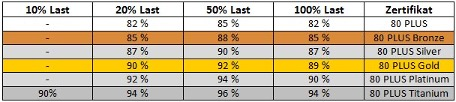
\includegraphics{80plus.jpg}
    \caption{Bedeutung 80-Plus Zertifikate}
\end{figure}

\textbf{Effizienz:}
Effizienz (oder Wirkungsgrad) gibt an, wie viel des verbrauchten Stroms tatsächlich dem Computer zur Verfügung steht.


\subsubsection{Speichermedien}

\begin{outline}
    \1 HDD
    \2 \textbf{H}ard \textbf{D}isk \textbf{D}rive
    \2 Daten werden magnetisch auf sich drehenden Platten gespeichert
    \2 Bestehen aus dem zu beschreibendem Medium, einem Schrittmotor und einem am Zugriffsarm befestigten Lese- und Schreibkopf
    \2 Üblicherweise in 2,5 Zoll (Für Notebooks) und 3,5 Zoll (für Desktop Rechner) verfügbar
    \2 Anschluss mit SATA-Kabel für Datenversorgung und SATA-Kabel für Stromversorgung
    \2 Sollten nicht dauerhaft einem starken magnetischen Feld ausgesetzt werden
    \2 Da die Platte in der HDD sehr schnell rotiert (bis zu 10000 rpm) sollte die vorgeschriebene Einbaulage beachtet werden
    \2 Reagiert empfindlich auf mechanische Einflüsse, daher sollten Erschütterungen vermieden werden
    \1 SSD
    \2 \textbf{S}olid \textbf{S}tate \textbf{D}rive
    \2 Daten werden auf Halbleiterchips gespeichert
    \2 Arbeitet ohne bewegliche Teile
    \2 Unempfindlich gegenüber mechanischen Stößen
    \2 Wesentlich höhere Lese- und Schreibraten als bei HDD möglich
    \2 Gängige Formate: 2,5 Zoll, M.2
    \2 Anbindung über SATA, PCI oder NVMe (PCI-Variante)
\end{outline}

\textbf{Fachbegriffe und Spezifikationen:}

\begin{table}[H]
    \begin{tabular}{|p{0.3\textwidth}|p{0.7\textwidth}|}
        \hline

        \textbf{Bauformen}                                                                  & 1,8 Zoll (selten – bei SSDs), 2,5-Zoll (SSD), 3,5 Zoll (HDD)

        \\\hline

        \textbf{Festplattenperformance}                                                     & Abhängig von den Zugriffszeiten, Datentransferrate und der Leistung der Schnittstelle. Bei HDDs außerdem Latenzen des Lese- und Schreibkopfes und die RPM der Festplatte relevant.
        \newline\textrightarrow\space Details siehe Aufgaben!

        \\\hline

        \textbf{Umdrehungsgeschwindigkeiten}                                                & Gibt an, wie schnell sich die Platte einer HDD maximal dreht. Angabe in RPM zwischen 5400 und 10000.

        \\\hline

        \textbf{Datentransferrate}                                                          & Hierfür sind die interne Anschlussweise (PCI-E oder SATA) und die Art der Festplatte entscheidend.

        \\\hline

        \textbf{Cache}                                                                      & Wie CPUs verfügen Festplatten über hoch performante Zwischenspeicher um Vorgänge wie das Entpacken oder Kopieren von Dateien zu beschleunigen.
        \newline Bei normalen Festplatten sind 16 bis 64 MB-Cache ausreichend. Bei hohen Leistungsanforderungen sollten es 64 bis 128 MB sein.

        \\\hline

        \textbf{Self-Monitoring, Analysis and Reporting Technology (SMART bzw. S.M.A.R.T.)} & Industriestandard zur Überwachung von Festplattenlaufwerken (HDD) und Solid-State-Drives (SSD) und dient der Vorhersage eines möglichen Ausfalls des Speichermediums. Es werden dabei die Werte verschiedener Sensoren mit Hilfe von unterschiedlichen Parametern ausgewertet.

        \\\hline
    \end{tabular}
\end{table}

\textbf{Pro und Contra – SSD und HDD}

\begin{table}[H]
    \centering
    \begin{tabular}{|p{0.2\textwidth}|p{0.25\textwidth}|p{0.25\textwidth}|p{0.25\textwidth}|}
        \hline
            & Pro & Contra & Einsatzzwecke \\\hline
        HDD &
        Günstiger als SSD
        \newline Mehr Speicherplatz möglich
        \newline Bessere Möglichkeit zur Datenwiederherstellung
            &
        Langsamer als SSD
        \newline Können laut werde
        \newline Anfällig gegenüber mechanischen Einwirkungen von außen
        \newline Höherer Stromverbrauch
            &
        Langfristigere Datenhaltung ohne Zugriffe (SSDs verlieren nach einer bestimmten Zeit ohne Strom ihre Daten)
        \newline Große Datenmengen speichern
        \newline Viele Lese-/Schreibzugriffe

        \\\hline

        SSD &
        Keine mechanischen Teile \textrightarrow\space robuster, geräuschlos
        \newline Schnell
        \newline Leicht
        \newline Effizient/Geringer Energiebedarf
            &
        Kosten
        \newline Nicht so viel Speicherplatz möglich
        \newline Schlechte Datenwiederherstellungsmöglichkeiten als bei einer HDD
            &
        Mobile Geräte
        \newline Vorteilhaft, wenn schnelle Zugriffszeiten relevant sind (z.B. Betriebssysteme oder Anwendungen, die häufig verwendet werden müssen)

        \\\hline
    \end{tabular}
\end{table}

\subsubsection{Dateisysteme und Formatierung}

Um auf einem Laufwerk Daten zu speichern, muss es zuerst formatiert werden. Dabei werden Strukturen geschaffen, die es dem Betriebssystem ermöglichen Daten auf dem Träger zu verwalten.

Bei Festplatten gibt es folgende Formatierungsschritte:
\begin{enumerate}
    \item Low-Level-Formatierung – LFF
    \item Erzeugung von Partitionen
    \item Logische Formatierung der Partitionen
          Häufig meint „Formatieren“ nur den letzten Schritt.
\end{enumerate}


\textbf{Low Level Formatierung bei HDDs:}
\begin{outline}
    \1 Erfolgt meist durch den Hersteller
    \1 Es werden auf die Plattenoberfläche eine Struktur aus logischen Spuren (tracks) und Sektoren (sectors) geschaffen
    \1 Die Anzahl der Spuren ist abhängig vom physikalischen Aufbau der Platte und sollte nachträglich nur von erfahrenen Usern mit speziellen Programmen geändert werden
    \1 Eine Spur ist ein schmaler, ringförmiger Streifen auf dem später die Daten gespeichert werden
    \1 Die Spuren werden auf jeder Plattenseite bei Spur null beginnend durchnummeriert
    \1 Spuren der gleichen Spurnummer gehören zu einem Zylinder
    \1 Jede Spur ist in Sektoren unterteilt. Sektoren sind die kleinste mögliche Speichereinheit einer Festplatte
    \1 Mehrere Sektoren ergeben zusammen ein Cluster
    \1 Ein Cluster ist der kleinste Speicherbereich eines Dateisystems
\end{outline}

\textbf{Aufbau bei SSDs:}
\begin{outline}
    \1 Für NAND-SSDs gelten folgende Zurechnungseinheiten:
    \2 Cells \textrightarrow\space Pages \textrightarrow\space Blocks \textrightarrow\space Planes
    \1 Ein Block ist die kleinste Struktur, die bei einer SSD gelöscht werden kann.
    \1 Anstelle der LLF gibt es bei SSDs das \textbf{Secure Erase}
    \1 Beim Secure Erase werden alle Bits der Speicherzellen auf 0 gesetzt
\end{outline}


\textbf{Partitionierung}
Eine Partition ist ein logisch selbständiger Teil einer Festplatte, der wie eine physisch separate Einheit funktioniert, vom Betriebssystem aus separates Laufwerk angesprochen wird und sich durch ein Dateisystem nutzen lässt.

Vorteile von Partitionierung:
\begin{outline}
    \1 Einfachere Organisation
    \1 Partitionen können einzeln formatiert werden
    \1 Betriebssystem kann einfach neu installiert werden
    \1 Mehrere Betriebssysteme möglich
    \1 Effizientere Suche nach Dateien
    \1 Einfachere logische Formatierung (z.B. verschiedene Dateisysteme)
\end{outline}

Nachteile von Partitionierung:
\begin{outline}
    \1 Ggf. Verschwendung von Speicherplatz
    \1 Falsches Gefühl von Sicherheit (Ausfall der Festplatte, Viren, etc.)
    \1 Unübersichtlich bei großer Anzahl von Partitionen
    \1 Kopieren/Verschieben von Dateien über Partitionen hinweg relativ langsam
\end{outline}

\subsubsection{Erweiterungskarten}
Viele Funktionen, die früher nur mit zusätzlichen Erweiterungen nachrüstbar waren sind heute auf dem Mainboard implementiert (z.B. Sound-, oder Netzwerkfunktionen). Das Nachrüsten mit zusätzlichen Karten ist daher nur dann erforderlich, wenn man beispielsweise eine qualitativ bessere Leistung erzielen möchte oder besondere Funktionen benötigt.

Der Anschluss von Erweiterungskarten erfolgt meist über einen PCIe-Slot auf dem Mainboard.

\subsubsection{Peripheriegeräte}
Peripherie-Geräte sind alle Geräte, die nach dem EVA-Prinzip zur Ein- und Ausgabe der Daten genutzt werden. Zu den gängigen Peripherie-Geräten gehören unter anderem:
\begin{outline}
    \1 Tastatur
    \1 Maus
    \1 Bildschirm
    \1 Lautsprecher/Headset
    \1 Drucker/Scanner
\end{outline}

\textbf{Eingabeeinheiten}
Tastatur und Maus gehören zu den klassischen Eingabeeinheiten. Bei der Anschaffung sollte auf Ergonomie und die nötigen Rahmenbedingungen geachtet werden.

Neben den klassischen Eingabeeinheiten gibt es außerdem unterschiedliche Branchenlösungen wie Zeichen-Tablets oder 3D Scanner.

\textbf{Ausgabeeinheiten – zentrale Einheit ist der Bildschirm}
Der Monitor ist die wichtigste Ausgabeeinheit.

Heutige Bildschirme werden als Liquid-Crystal-Displays (LCD) angeboten. Hersteller setzten bei LCD-Monitoren auf LED-Technik, da sie sehr energiesparend ist und die LEDs eine Hintergrundbeleuchtung er-möglichen.

Als Standardgröße und normale Eigenschaften für Office-Monitore gelten häufig 27-Zoll, Full-HD, eine Reaktionszeit von 4-8 ms und 60 Hz.

\textbf{Eigenschaften im Überblick}
\begin{longtable}{|p{.2\textwidth}|p{.8\textwidth}|}
    \hline
    \textbf{LCD-Technologie}           &
    LCD ist die derzeitige Bautechnologie von Monitoren, die spezielle Verarbeitungsart Thin-Film-Transistor-Technologie (TFT) bei LCD-Monitoren liegt auch LCD-Fernsehern zugrunde.

    Flüssigkristalle eines LCD-Monitors bilden die einzelnen Bildpunkte (Pixel) des Monitors. Ein Pixel besteht aus drei Farbfiltern (Rot, Grün, Blau), die rückseitig beleuchtet werden. Die Art der Lichtpolarisation durch die Kristalle unterscheidet sich jedoch nach den Panel-Typen.
    \begin{outline}
        \1 TN: preisgünstig und schnelle Reaktionszeit, relativ energiesparsam, aber schlechte Blickwinkeldichte.
        \1 VA: gute Bildqualität aber geringe Reaktionszeit
        \1 IPS: sehr gute Bildqualität und gute Blickwinkeldichte aber höhere Anschaffungskosten
    \end{outline}
    \\\hline

    \textbf{Größen / Seitenverhältnis} &
    Größenangaben erfolgen in Zoll (Bildschirmdiagonale), typisch sind 24 oder 27 Zoll bei einem Seitenverhältnis von 16:9. Curved-Bildschirme sind dagegen häufig etwas größer und sind auch im 21:9 Seitenverhältnis zu kaufen.
    \\\hline

    \textbf{Ergonomie}                 &
    Da Monitore häufig über längere Zeiträume hinweg den zentralen Punkt eines Arbeitsplatzes bilden, ist die ergonomische Ausrichtung von hoher Wichtigkeit.

    Eine Rolle spielt neben der Größe, dem dazu passenden Abstand vom Monitor (Diagonale * 1,6) und der Krümmung des Monitors auch die Eigenschaft den Monitor horizontal zu neigen (Tilt), vertikal zu drehen (Swivel) oder horizontal zu drehen bzw. die Höhe zu verstellen (Pivot).

    Dazu gibt es außerdem noch verschiedene Filter (z.B. Blaufilter) die die Augen vor einer Ermüdung schützen sollen.
    \\\hline

    \textbf{Reaktionszeit}             &
    Die Reaktionszeit beim Monitor gibt an wie viel Zeit die Pixel des Displays benötigen, um einen Farbwechsel vorzunehmen. Üblicherweise wird ein Farbwechsel zwischen zwei Grautönen (Grey to Grey) oder Schwarz und Weiß gemessen. Typisch sind Zeiten unter 10 ms wobei gilt, kleiner desto besser.
    \\\hline

    \textbf{Bildwiederhol-}              \\\textbf{frequenz}&
    Gibt an, wie viele Einzelbilder (Refresh) pro Sekunde vom Monitor dargestellt wer-den können. Die meisten Monitore liefern eine Bildwiederholfrequenz von 60 Hz. Das bedeutet, dass pro Sekunde 60 Einzelbilder vom Monitor dargestellt werden können. Daneben gibt es z.B. auch 75, 120 oder 144 Hz. Die treusten Monitore haben bis zu 240 hz.
    \\\hline

    \textbf{Auflösung}                 &
    Richtet sich nach der Größe und dem Seitenverhältnis eines Monitors.

    Gängig sind 1920 x 1080 (HD), 2560 x 1440 (WQHD) oder 4.096 x 2.160 Pixeln (4k).

    \\\hline
\end{longtable}

\textbf{Ausgabeeinheiten – Drucker unterscheiden}

\begin{longtable}{|p{.3\textwidth}|p{.7\textwidth}|}
    \hline

    \textbf{Arbeitsplatz/Desktop Drucker} &
    Werden häufig im kleineren Rahmen im geschäftlichen Bereich eingesetzt. Häufig werden nur einzelne/wenige Arbeitsplätze direkt angebunden um Weg/Zeit zu sparen.

    Häufig handelt es sich um Multifunktionsgeräte mit Drucker/Scanner/Kopierer/Fax.
    \\\hline

    \textbf{Abteilungsdrucker}            &
    Für größere Druckvolumen oder Spezialaufträge werden gerne Abteilungsdrucker eingesetzt. Diese sind auf 10000 Ausdrucke und mehr im Monat ausgelegt und bieten den Druck schnell und günstig.

    Außerdem können solche Geräte bspw. im Duplex-Verfahren (Beidseitig) drucken und verfügen ebenfalls über Kopie/Scan/Fax Optionen.

    Häufig ist die Anmeldung über eine Codekarte oder einen Login notwendig.
    \\\hline

    \textbf{Mobile Drucker}               &
    Mobile Drucker sind besonders für Mitarbeiter im Außendienst relevant. Der Druck ist langsam und teuer, dafür sind die Drucker sehr mobil, um bspw. Rechnungen direkt drucken zu können.


    \\\hline
\end{longtable}
\break
\textbf{Drucksysteme im Vergleich}

Tinten- oder Inkjet-Drucker:
\begin{table}[H]
    \begin{tabular}{|p{.5\textwidth}|p{.5\textwidth}|}
        \hline
        Vorteile & Nachteile
        \\\hline

        \begin{outline}
            \1 Druckt auf CDs/DVDs, Spezialpapier.
            \1 Fotodrucke haben hervorragende Qualität.
            \1 Es gibt spezielle Tintenstrahldrucker, mit speziellen Fotofarben.
            \1 Keine Aufwärmphase notwendig.
            \1 Keine Hitzeabgabe.
            \1 Im Betrieb (und vor allem auch Stand-By) leiser.
            \1 Günstigere Anschaffungskosten.
            \1 Geringerer Stromverbrauch.
            \1 Keine Feinstaubbelastung.
            \1 Eher für Wenigdrucker geeignet (unter 200 Seiten pro Monat)
        \end{outline}
                 &
        \begin{outline}
            \1 Kürzere Lebensdauer.
            \1 Benötigt hochwertiges (und teures) Druckerpapier.
            \1 Druckpatronen sind sehr teuer.
            \1 Tintenpatronen/Druckkopf trocknen nach längerer Zeit ohne Benutzung ein.
            \1 Spülen mit teurer Druckertinte erhöht die Druckkosten noch zusätzlich.
            \1 Niedrigere Druckgeschwindigkeit.
            \1 Ausdrucke aufgrund von schlechter UV-Beständigkeit und fehlender Feuchtigkeitsresistenz nicht so lange haltbar.
        \end{outline}
        \\\hline
    \end{tabular}
\end{table}


Laserdrucker:
\begin{table}[H]
    \begin{tabular}{|p{.5\textwidth}|p{.5\textwidth}|}
        \hline
        Vorteile & Nachteile
        \\\hline

        \begin{outline}
            \1 Geringe Kosten pro gedruckter Seite.
            \1 Höhere Druckgeschwindigkeit.
            \1 Gut geeignet für Textdrucke wie Dokumente und E-Mails.
            \1 Nicht so anspruchsvoll bezüglich der Papierqualität, es kann z. B. günstiges (und umweltschonendes) Recyclingpapier verwendet werden.
            \1 Hohe Schriftrandschärfe (= scharfe und klare Textausdrucke).
            \1 Hohe Farbtiefe.
            \1 UV- und Feuchtigkeitsresistent. Damit wischfest und es kommt nicht zum Ausbleichen.
            \1 Vor allem für Vieldrucker (Büro und Firmen) geeignet. Rechnet sich ab ca. 200 gedruckten Seiten pro Monat.

        \end{outline}
                 &
        \begin{outline}
            \1 Geringe Druckschärfe und deshalb nicht geeignet für das Drucken von Bildern und Fotos.
            \1 Höherer Anschaffungspreis als Tintenstrahldrucker.
            \1 Höhere Schadstoff- / Feinstaubemissionen.
            \1 Benötigt Zeit zum Aufwärmen.
            \1 Wärme- und Geräuschentwicklung.
            \1 Höherer Stromverbrauch.
        \end{outline}
        \\\hline
    \end{tabular}
\end{table}


\subsection{Dateisicherung - für ASP1 wahrscheinlich nur oberflächlich}

\subsubsection{RAID-Systeme}

Bei einem RAID-System handelt es sich um einen logischen Zusammenschluss mehrerer einzelner physischer Massenspeicher, wie z.B. HDD oder SSD Festplatten. In der Regel erreicht man dadurch eine Steigerung der Geschwindigkeit der Schreib- und Lesezugriffe oder die Verbesserung der Datensicherheit.

Ein RAID kommt also immer dann zum Einsatz, wenn folgende Ziele erreicht werden sollen:
\begin{itemize}
    \item durch Datenredundanz die Ausfallsicherheit und damit Datensicherheit verbessern.
    \item durch die Steigerung der Transferraten die Geschwindigkeit (Performance) steigern.
    \item oder beides zusammen.
\end{itemize}



\subsubsection{Backup Verfahren}

Bei einem Backup wird die Sicherheit der Daten durch das Anlegen einer separaten, unabhängigen Kopie erhöht. Bei einem Verlust der Originaldaten kann man auf die Kopie zugreifen und die Daten somit wieder-herstellen. Hierdurch hilft ein Backup auch in solchen Situationen, in denen ein RAID System versagt.

\textbf{Verschiedene Backup Verfahren:}
\begin{outline}
    \1 Inkrementelles Backup
    \1 Differentielles Backup
    \1 Vollbackup
\end{outline}

Die optimale Backup-Methode muss je nach Anwendungsfall gewählt werden. Häufig macht eine Kombination aus allen drei Methoden am meisten Sinn. Zum Beispiel kann ein wöchentliches Vollbackup erfolgen und zusätzlich jeden Tag ein inkrementelles Backup, um das Datenaufkommen niedrig zu halten und mit den entsprechenden Sicherungen die Daten schnell und zu verschiedenen Zeitpunkten wiederherzustellen.


\subsubsection{USV}

Eine USV ist ein Gerät, welches zwischen den Netzanschluss und den oder die Verbraucher geschaltet wird. Sie beinhaltet eine Pufferbatterie und kann daraus Strom liefern, wenn die Netzversorgung ausfällt.


\break

\end{document}